\documentclass[12pt]{article}
\usepackage{fontspec} % 字型
\setmainfont{Taipei Sans TC Beta}
\usepackage{xeCJK} % 字型
\setCJKmainfont{Taipei Sans TC Beta}
\usepackage[top=1cm, bottom=1cm, left=1cm, right=1cm]{geometry} % 頁面設定
% \usepackage{indentfirst} % 首行縮排
\renewcommand{\baselinestretch}{1.5}
\pagenumbering{gobble} % 無頁碼
\usepackage{enumitem} % 列表縮排
\usepackage{zhnumber} % 中文數字
\usepackage{graphicx}

\begin{document}

\section*{pA:搜尋元素}

\begin{itemize}[label={}, itemsep=0pt]
    \item 有 $n$ 個排序元素 $a_i$,對於 $k$ 個答詢 $b_i$ 輸出\textbf{是否在陣列 $a$ 裡面}。
    \item 測資範圍:$1 \leq n, k \leq 10^5, -10^9 \leq a_i, b_i \leq 10^9$
    \item 輸入順序:$n, a, b$
    \item 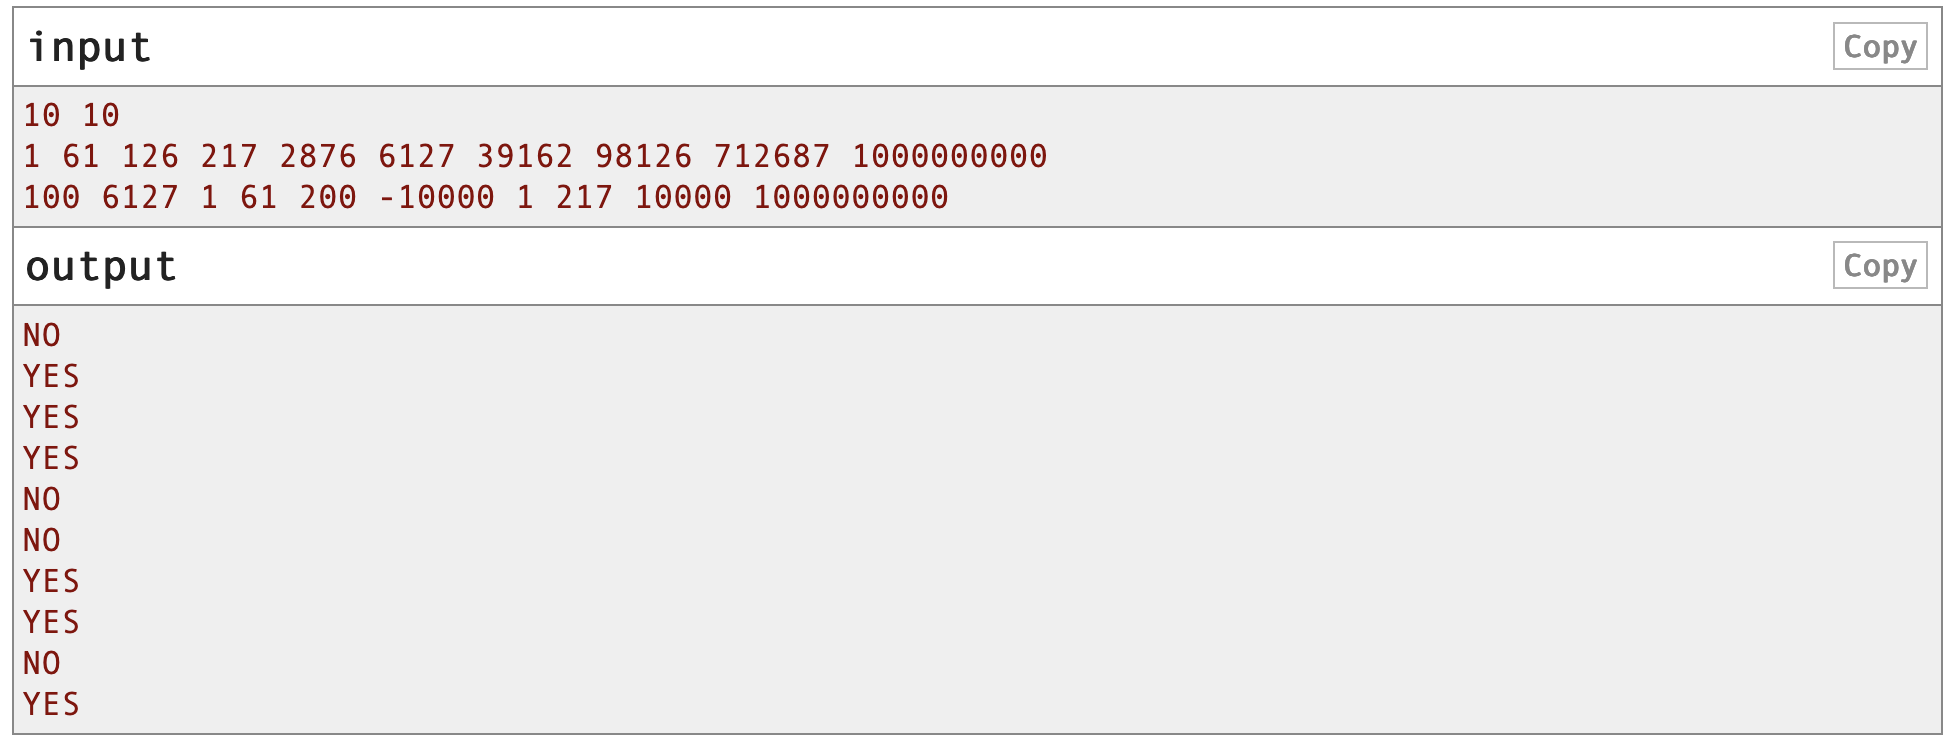
\includegraphics[width=15.0cm]{img/pA.png}
\end{itemize}

\section*{pB:不大於 k 的數}

\begin{itemize}[label={}, itemsep=0pt]
    \item 有 $n$ 個排序元素 $a_i$,對於 $k$ 個查詢 $b_i$ 輸出\textbf{不大於 $b_i$ 的最大數的索引值}(1-based),如果沒有就輸出 $0$。
    \item 測資範圍:$0 \leq n, k \leq 10^5, 2 \times -10^9 \leq a_i, b_i \leq 2 \times 10^9$
    \item 輸入順序:$n, k, a, b$
    \item 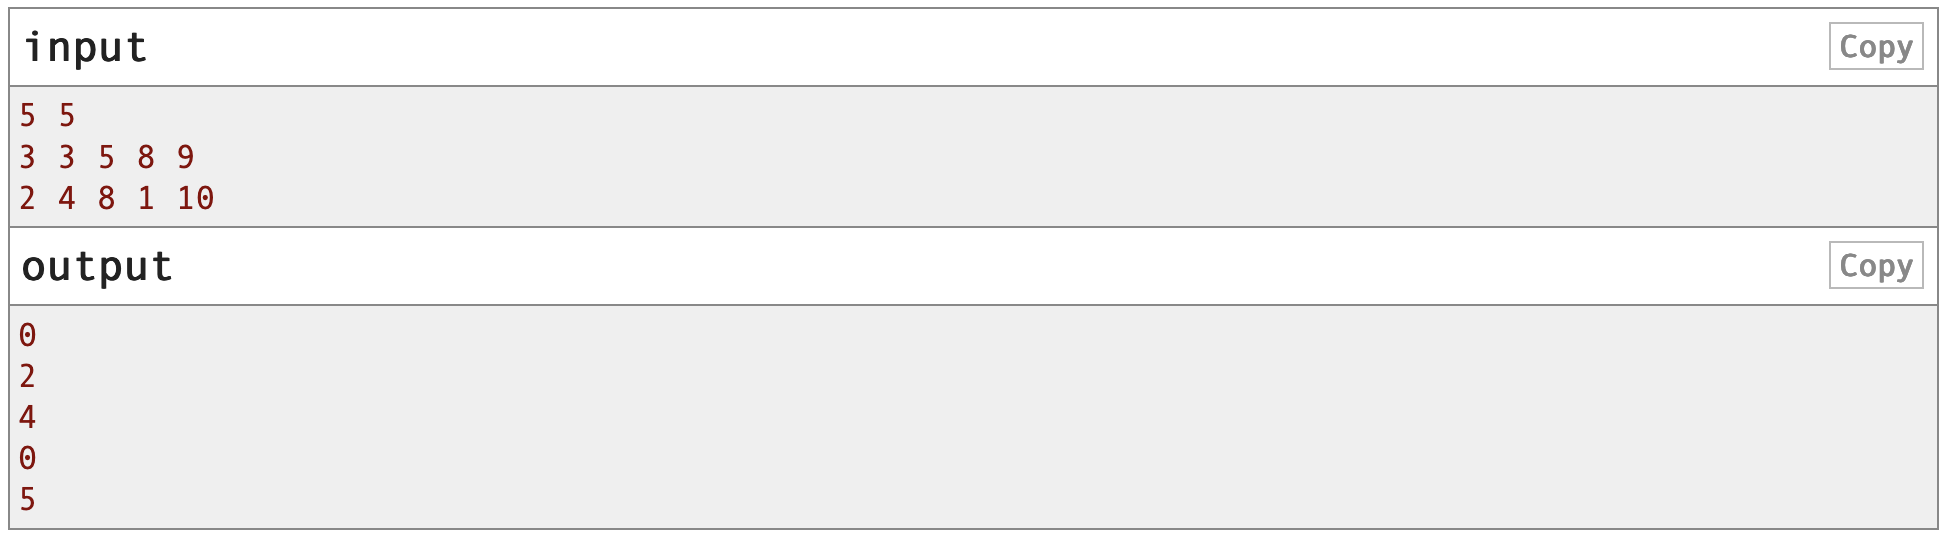
\includegraphics[width=15.0cm]{img/pB.png}
\end{itemize}

\section*{pC:不小於 k 的數}

\begin{itemize}[label={}, itemsep=0pt]
    \item 有 $n$ 個排序元素 $a_i$,對於 $k$ 個查詢 $b_i$ 輸出\textbf{不小於 $b_i$ 的最小數的索引值}(1-based),如果沒有就輸出 $n+1$。
    \item 測資範圍:$0 \leq n, k \leq 10^5, 2 \times -10^9 \leq a_i, b_i \leq 2 \times 10^9$
    \item 輸入順序:$n, k, a, b$
    \item 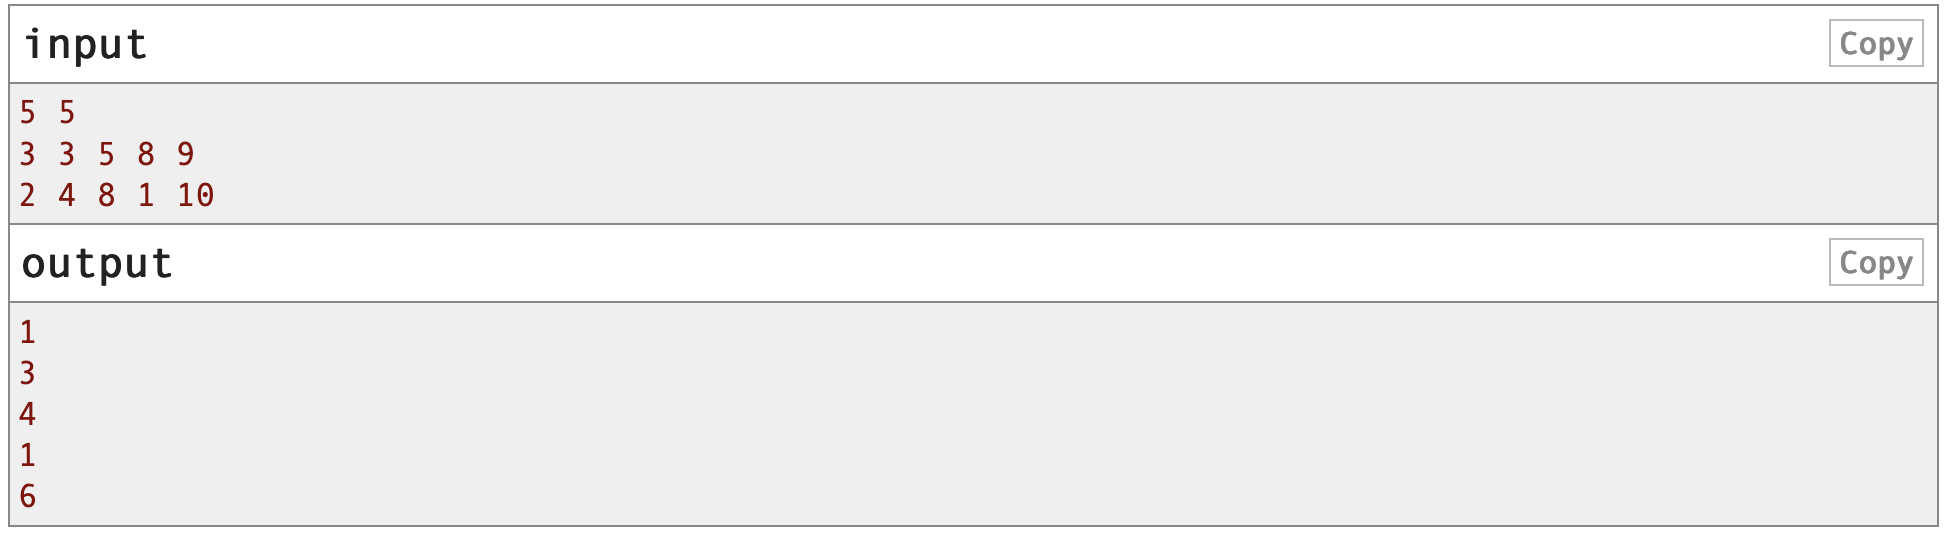
\includegraphics[width=15.0cm]{img/pC.png}
\end{itemize}

\section*{pD:區間數值數量}

\begin{itemize}[label={}, itemsep=0pt]
    \item 有 $n$ 個元素 $a_i$,對於 $k$ 個查詢 $L_i, R_i$ 輸出 $n$ 裡面\textbf{有多少數字在區間$[L_i, R_i]$內}。
    \item 測資範圍:$0 \leq n, k \leq 10^5, -10^9 \leq a_i, b_i \leq 10^9$
    \item 輸入順序:$n, a, k, l, r$
    \item 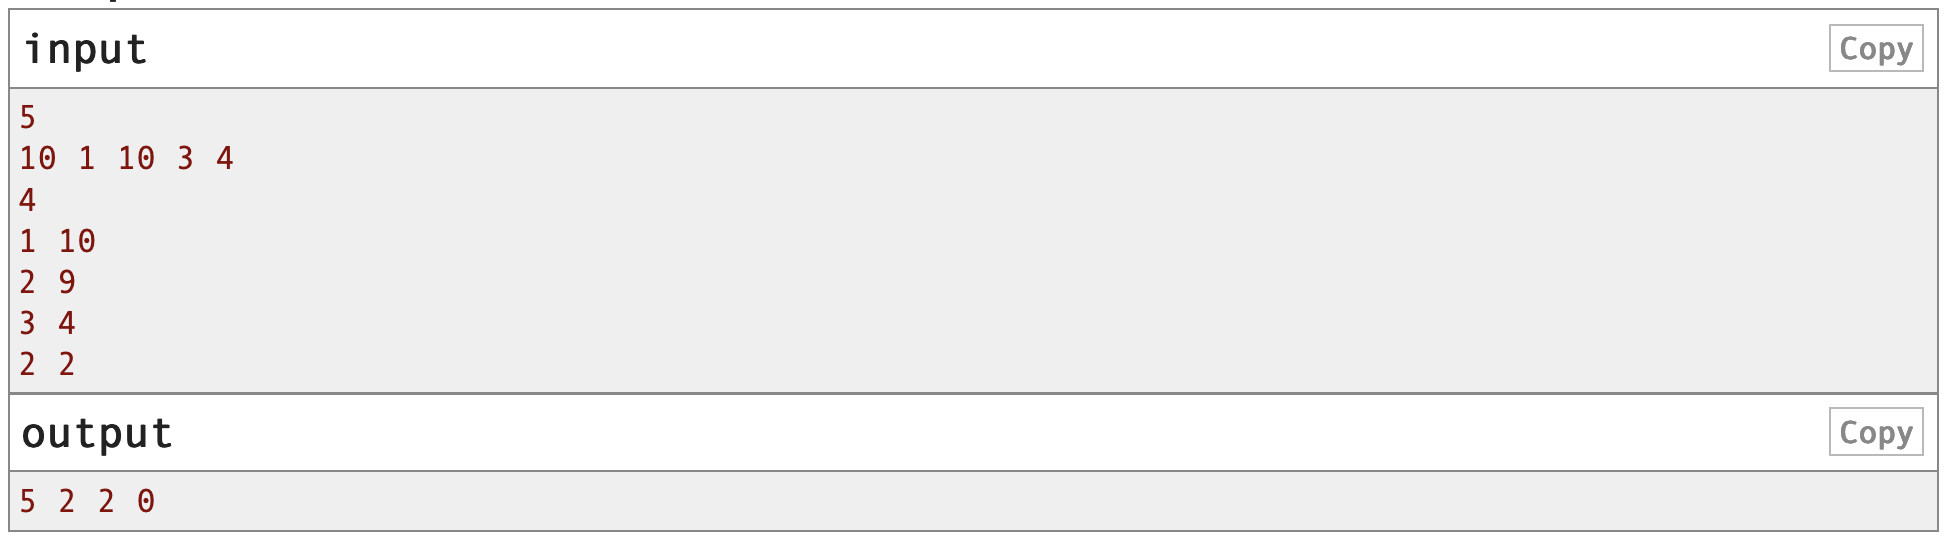
\includegraphics[width=15.0cm]{img/pD.png}
\end{itemize}

\section*{pE:貨物包裝}

\begin{itemize}[label={}, itemsep=0pt]
    \item 有 $n$ 長為 $w$ 寬為 $h$ 長方形貨物,請問\textbf{可以包裝所有貨物的最小正方形貨倉的邊長是多少},請注意,貨物不能旋轉。
    \item 測資範圍:$-10^9 \leq n, w, h \leq 10^9$
    \item 輸入順序:$w, h, n$
    \item 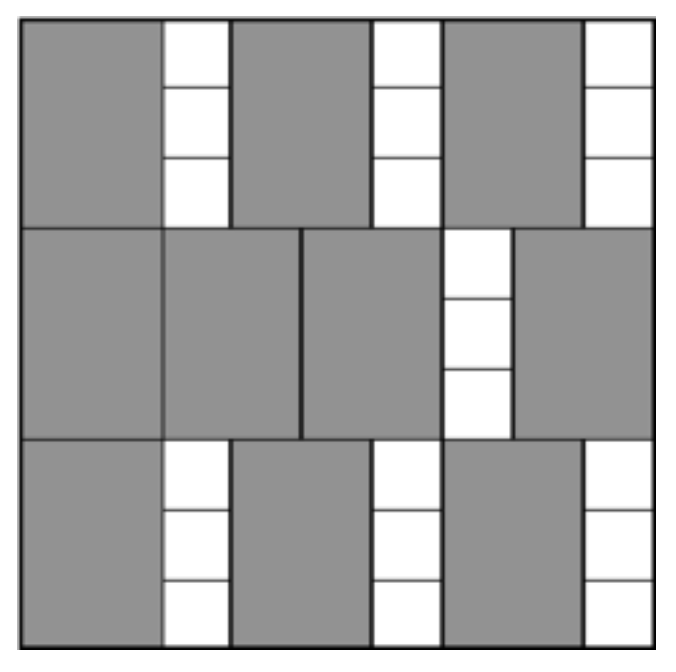
\includegraphics[width=4.0cm]{img/pE-1.png} 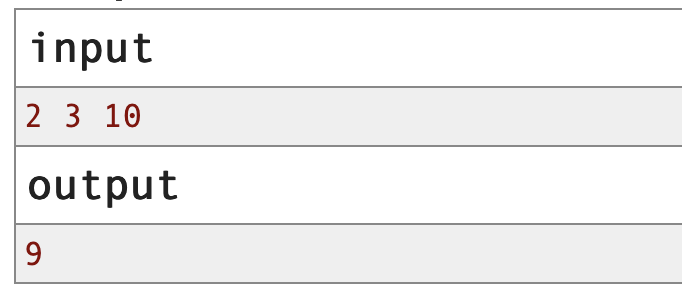
\includegraphics[width=8.0cm]{img/pE-2.png}
\end{itemize}

\section*{pF:機器排程}

\begin{itemize}[label={}, itemsep=0pt]
    \item 你有 $n$ 個機器,每個機器會使用 $k_i$ 單位時間生產一個物品,\textbf{輸出最少需要多少單位時間才能生產 $t$ 個貨物}。
    \item 測資範圍:$1 \leq n \leq 2 \times 10^5, 1 \leq t, k_i \leq 10^9$
    \item 輸入順序:$n, t, k$
    \item 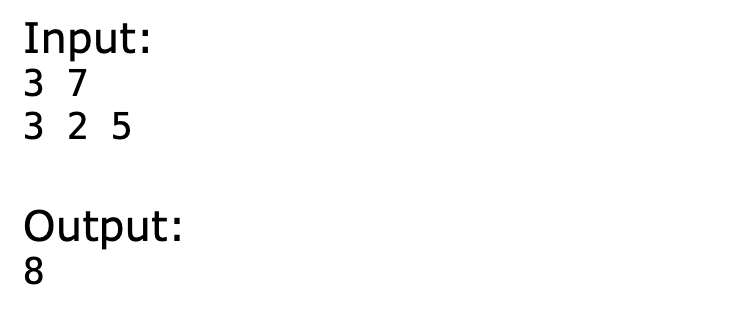
\includegraphics[width=6.0cm]{img/pF.png}
\end{itemize}

\section*{pG:乘法表}

\begin{itemize}[label={}, itemsep=0pt]
    \item 你有一個大小為 $n \times n$ 的乘法表 $a$,$a_{(i,\ j)}$ 的值為 $i \times j$,請你找出這個乘法表的中位數。
    \item 測資範圍:$1 \leq n \leq 10^6$ 且 $n$ 必定是奇數
    \item 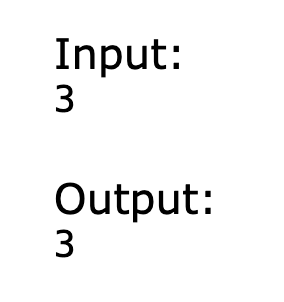
\includegraphics[width=3.0cm]{img/pG-2.png}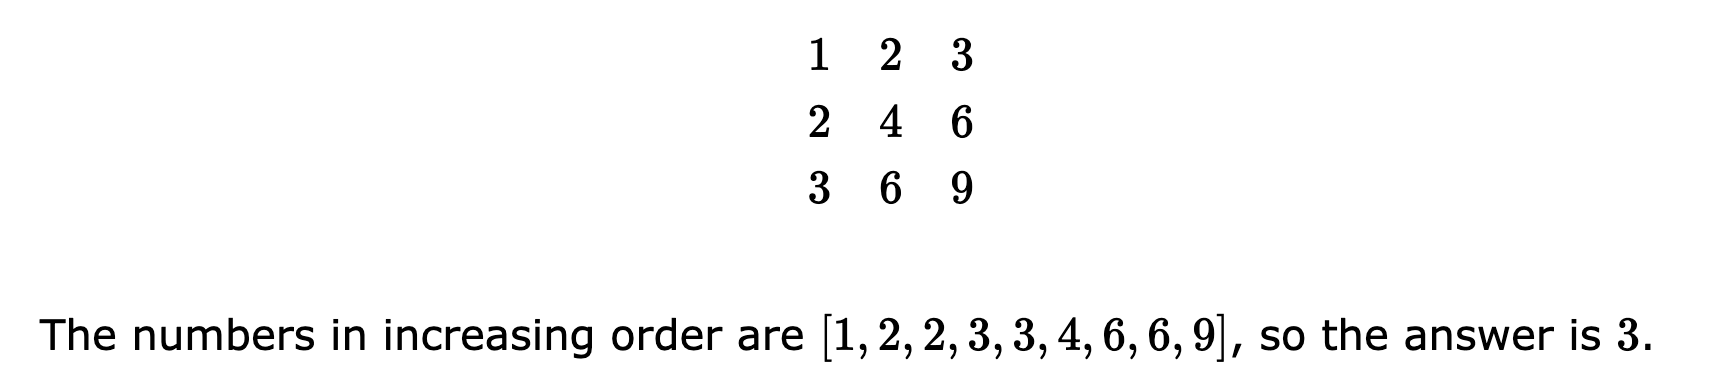
\includegraphics[width=12.0cm]{img/pG-1.png}
\end{itemize}

\section*{pH:第 k 小數對和}

\begin{itemize}[label={}, itemsep=0pt]
    \item 你有兩個大小為 $n$ 的陣列,對於所有可能的 $1 \leq i, j \leq n$ 的多重集 $a_i+b_j$,輸出第 $k$ 小的數對和。
    \item 測資範圍:$1 \leq n \leq 2 \times 10^5, 1 \leq k \leq n^2$
    \item 輸入順序:$n, k, a, b$
    \item 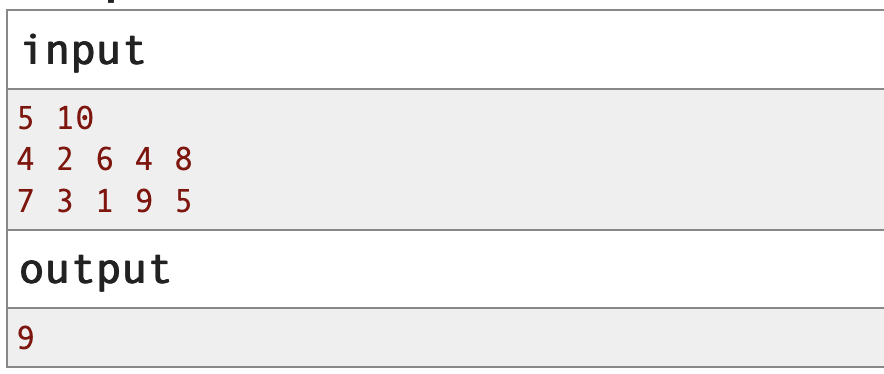
\includegraphics[width=8.0cm]{img/pH.png}
    \item 說明:多重集為 \{3, 5, 5, 5, 7, 7, 7, 7, 9, 9, 9, 9, 9, 11, 11, 11, 11, 11, 13, 13, 13, 13, 15, 15, 17\},第 10 小的數為 9
\end{itemize}

\end{document}